\documentclass[a4paper,11pt ]{xc_webpage_project}
\usepackage[utf8]{inputenc}
\usepackage[spanish,english]{babel}
\usepackage{graphicx}
\usepackage[labelsep=period]{caption}
\usepackage{parallel}
\usepackage{wrapfig} %% Wrapping text around figures.
\usepackage{caption}
\usepackage{subcaption}

\renewcommand{\titProject}{Pasarela sobre el río Isuela en Huesca}
\def\@anagramFont{\relax}
\renewcommand{\client}{Ayto. de Huesca}
\renewcommand{\dateProject}{2021}
\renewcommand{\location}{Huesca (España)}
\renewcommand{\widhtLeftCol}{0.50\textwidth} % normalmente no lo cambiaremos
\renewcommand{\widhtRightCol}{0.45\textwidth} % normalmente no lo cambiaremos


\begin{document}
\headerSpanish

\begin{Parallel}{\widhtLeftCol}{\widhtRightCol}
   \ParallelLText{
    En el año 2.009, el Ayuntamiento de Huesca promovió la construcción de una pasarela  para usos peatonal y ciclista   en la zona noreste de la ciudad. Dicha pasarela cruza el río Isuela  entre las calles Tenerías y Velódromo de Huesca, comunicando los barrios de Santo Domingo y el Perpetuo Socorro,  a la altura del Parque del Encuentro.  Se trata de una pasarela  de un solo vano y 24 m de luz, con un ancho total de 2,80 m. La solución estructural adoptada para el tablero consistió en dos jácenas metálicas longitudinales de sección I y vigas transversales arriostradas con diagonales, sobre las que apoya un forjado de chapa colaborante. El tablero apoya, mediante placas de neopreno, en dos cargaderos cimentados sobre zapatas.
   }
  
   \ParallelRText{
     \emph{In 2009, the Huesca City Council promoted the construction of a footbridge for pedestrian and cyclist use in the northeast area of the city. This footbridge crosses the Isuela River between Tenerías and Velódromo de Huesca streets, connecting the neighborhoods of Santo Domingo and Perpetuo Socorro, at the Parque del Encuentro. It is a 24 m single-spam footbridge, with a total width of 2.80 m. The structural solution adopted for the deck consisted of two I-section longitudinal steel girders and braced transversal beams with diagonals, on which a collaborating sheet metal floor rests. The deck rests, by means of neoprene plates, on two stub abutments founded on footings.}
   }
\end{Parallel}


  \begin{figure}[h]
  \begin{subfigure}[l]{\widhtLeftCol}
  \centering
  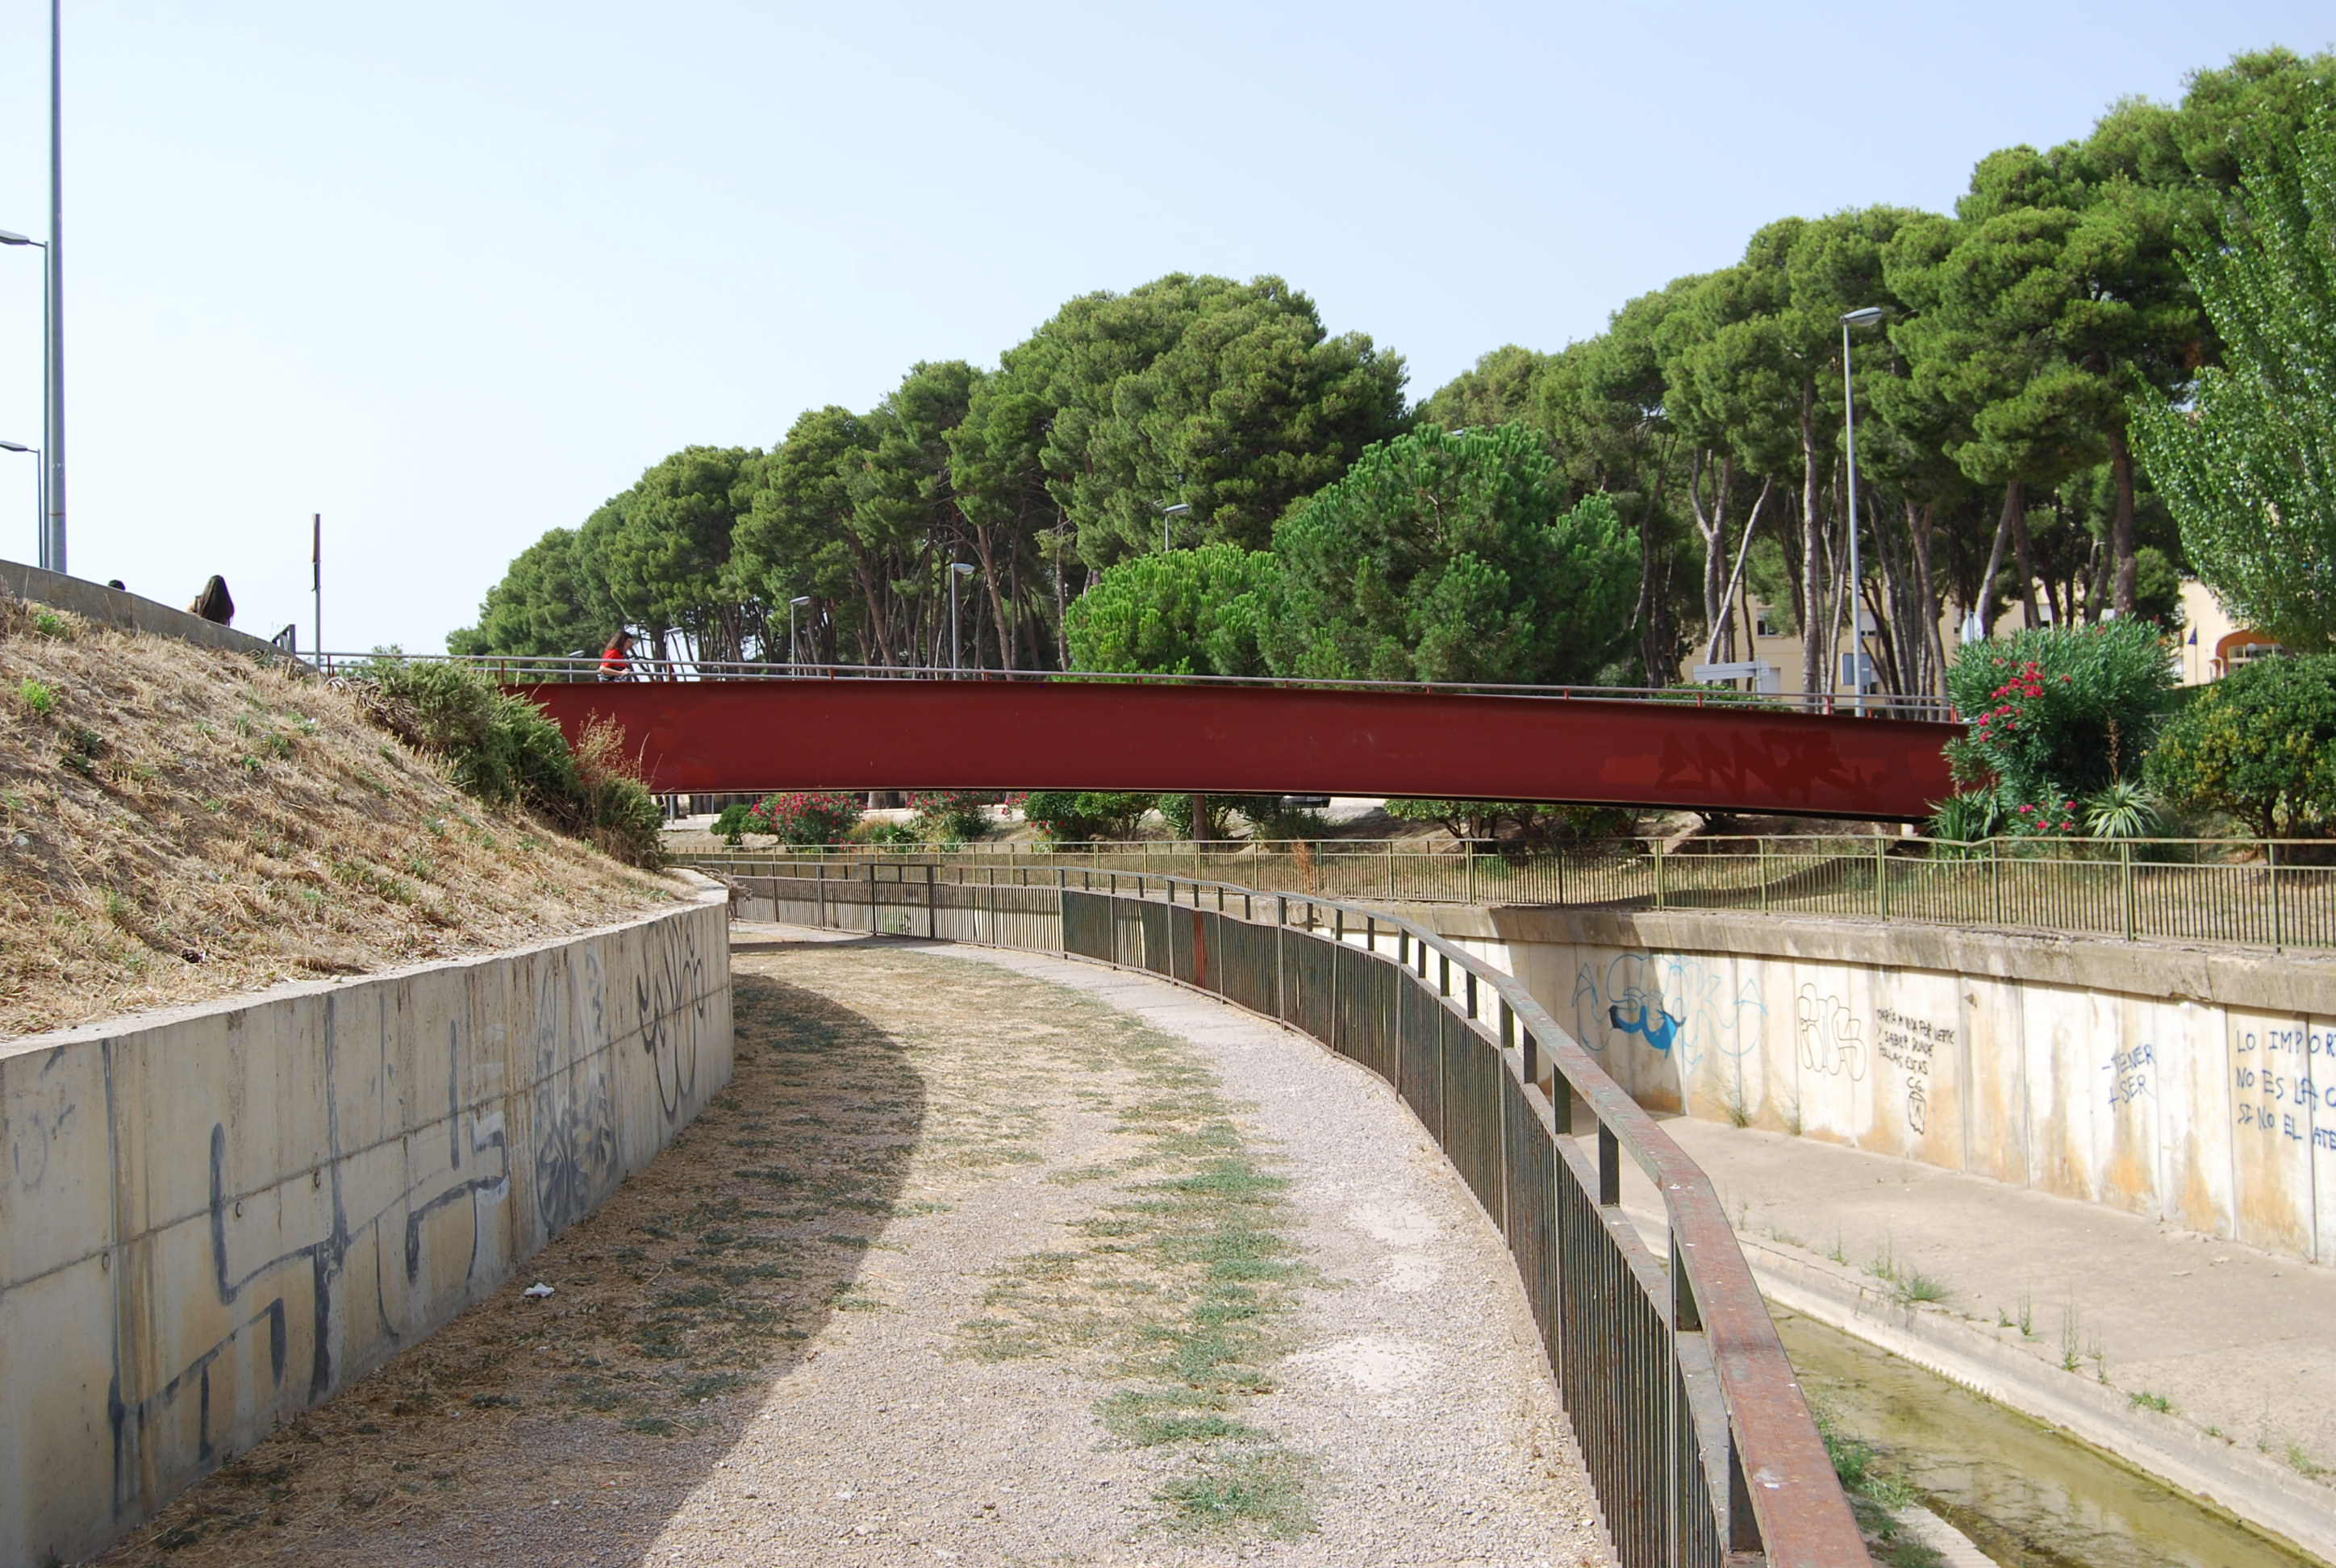
\includegraphics[width=\textwidth]{figures/DSC_0321}
  \caption{Vista de la pasarela desde la senda peatonal habilitada en la margen derecha del encauzamiento del río Isuela}
  \end{subfigure}
\hfill
  \begin{subfigure}[r]{\widhtRightCol}
  \centering
  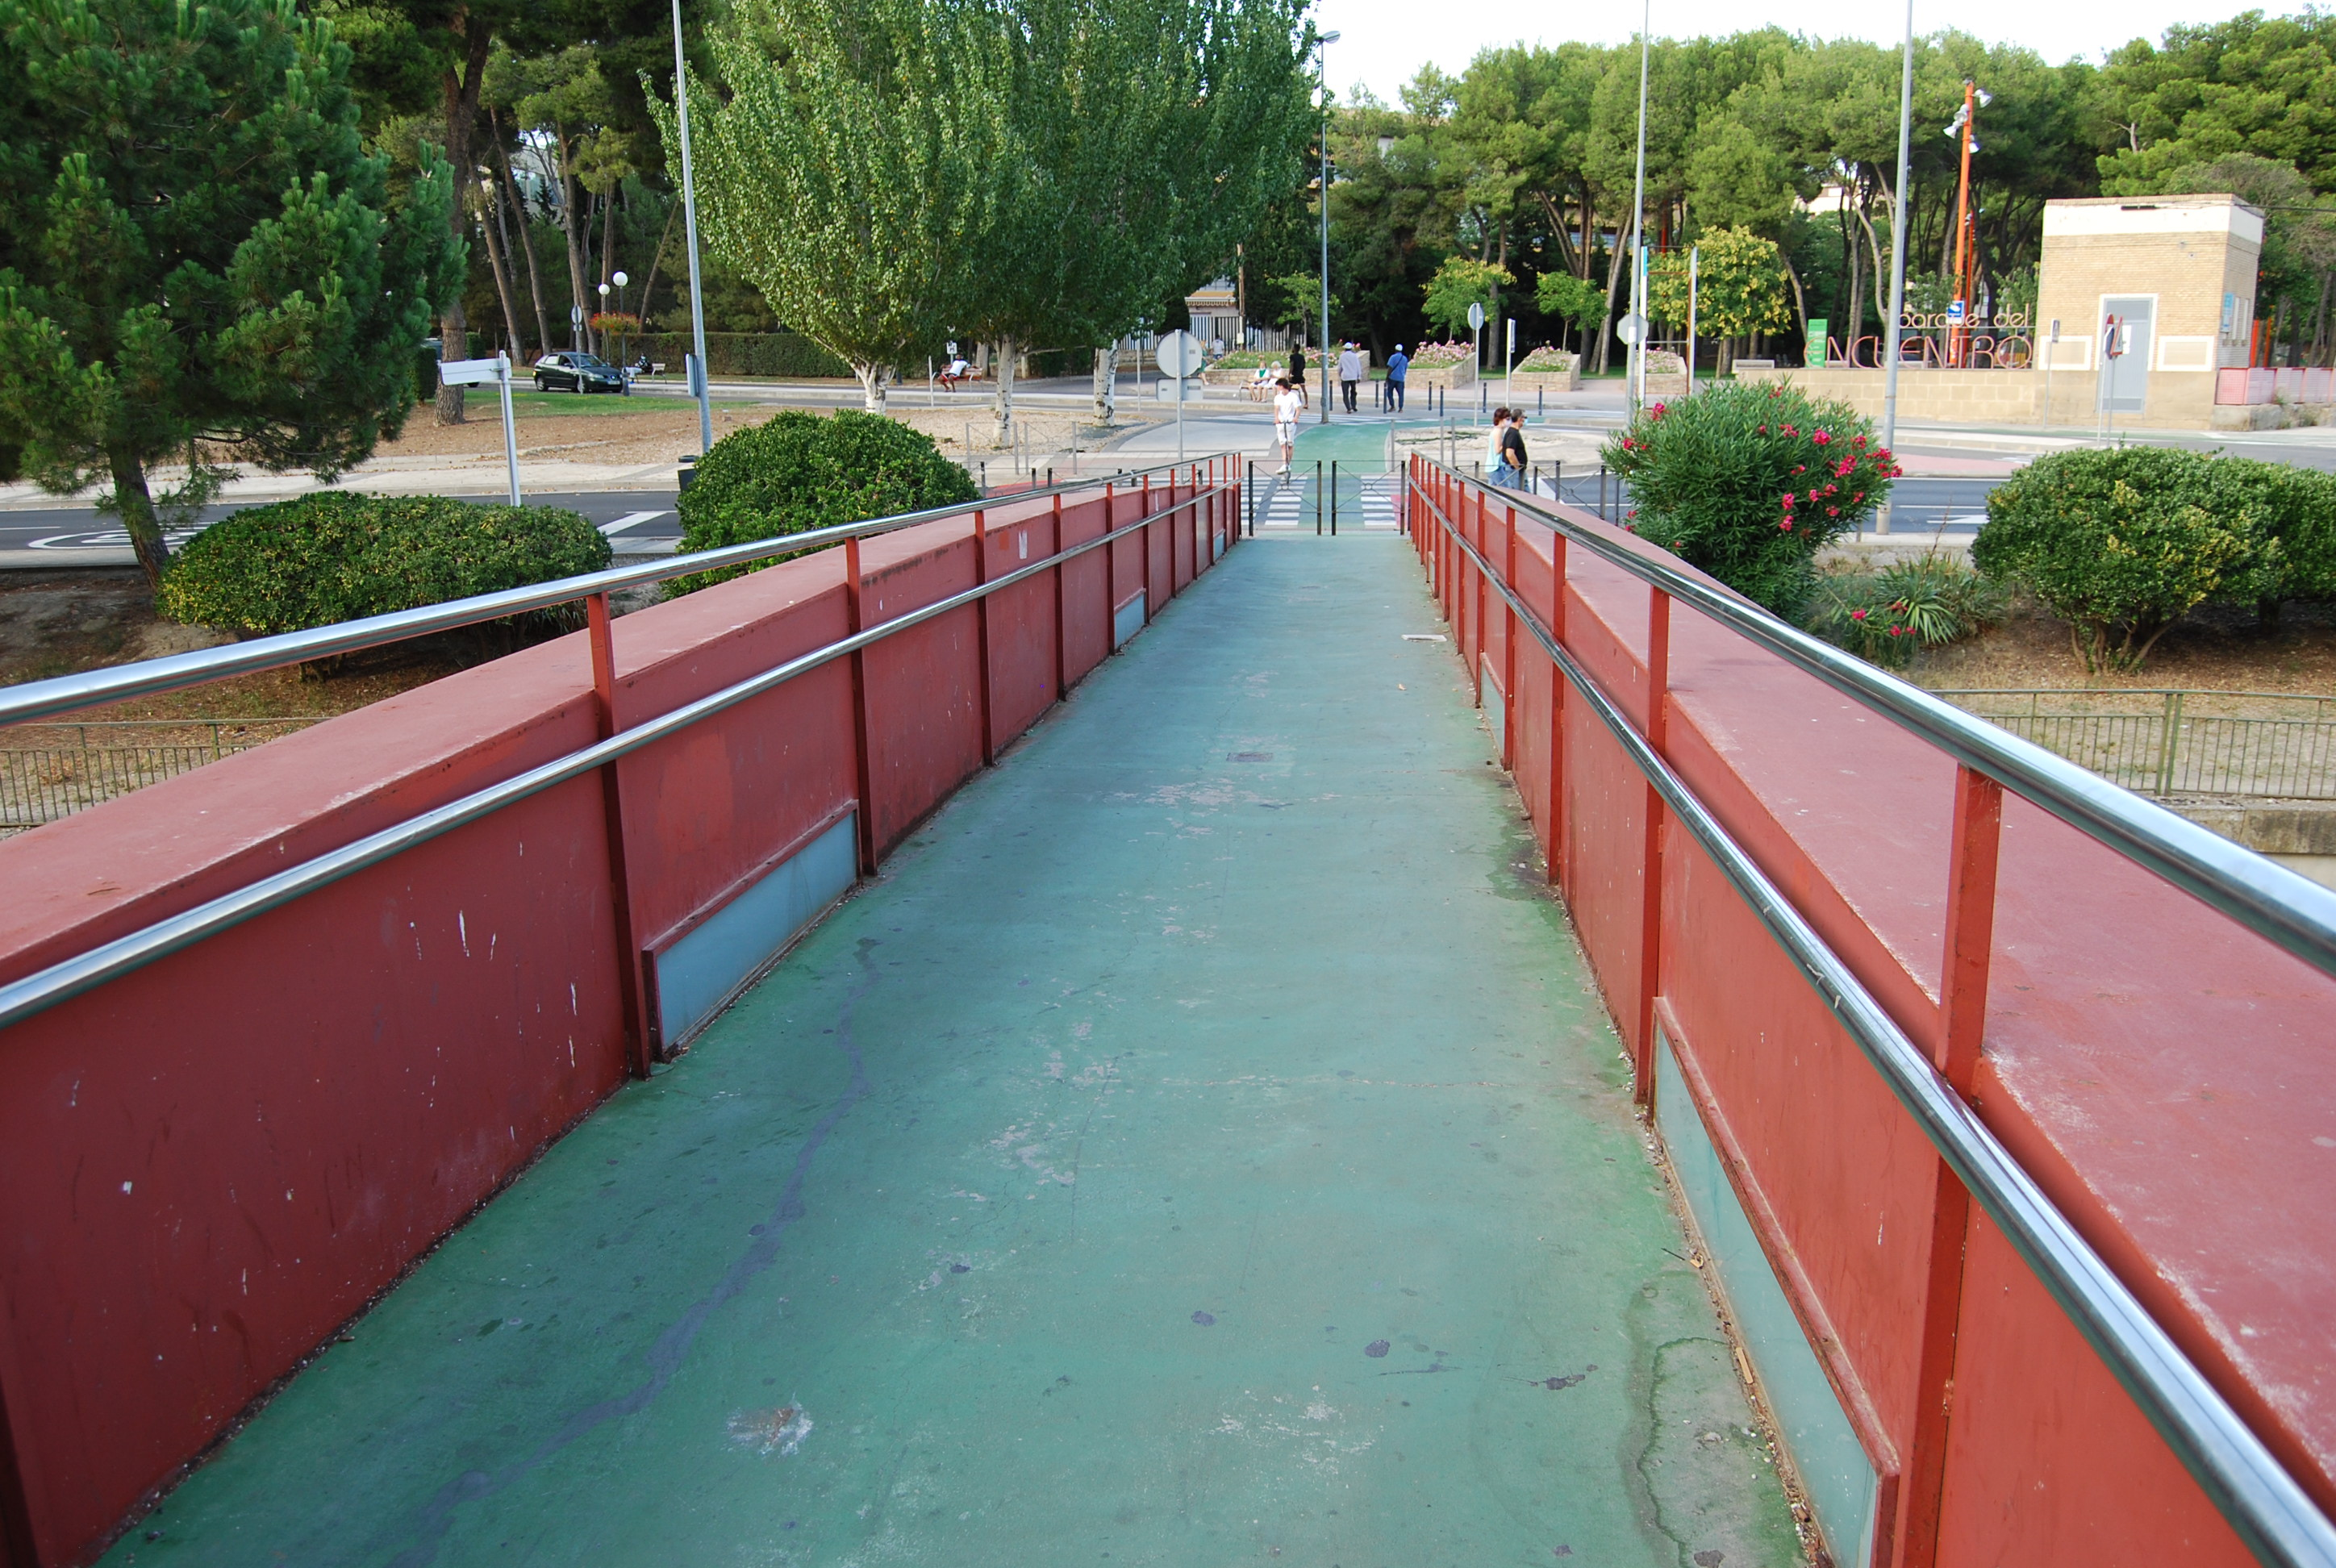
\includegraphics[width=\textwidth]{figures/DSC_0312}
  \caption{Acceso a la  pasarela desde margen derecha, en dirección al Parque del Encuentro}
  \end{subfigure}
  \end{figure}


\begin{Parallel}{\widhtLeftCol}{\widhtRightCol}
   \ParallelLText{
     XC ingeniería estructural recibió en 2.021 el encargo de redactar un Proyecto constructivo para rehabilitación de dicha pasarela. Durante las visitas de inspección realizadasa se observó un cuadro de patologıía en el tablero, afectando especialmente a la chapa colaborante del forjado. Ésta presentaba un grado de corrosión elevado, probablemente ocasionado por la falta de impermeabilidad del mismo, pues dicha corrosión se acusaba de manera más grave bajo las líneas de fisuras que se observan en la superficie del pavimento. En contraste, el estado de la estructura principal (jácenas y celosía metálica) era razonablemente bueno y los estribos-cargadero y aparatos de apoyo mostraban un buen estado de conservación.
   }
  
   \ParallelRText{
     \emph{XC structural engineering was commissioned in 2021 to draft a construction project for the rehabilitation of said footbridge. During the inspection visits carried out, a pathology was observed in the deck, especially affecting the collaborating sheet of the floor, which presented a high degree of corrosion, probably caused by its lack of impermeability, since that corrosion was more severe under the pavement cracks. In contrast, the steel main structure, abutments and  neoprene bearing pads were in a good state of preservation.   
     }
   }
\end{Parallel}

\begin{figure}[h]
  \begin{subfigure}[l]{\widhtLeftCol}
  \centering
  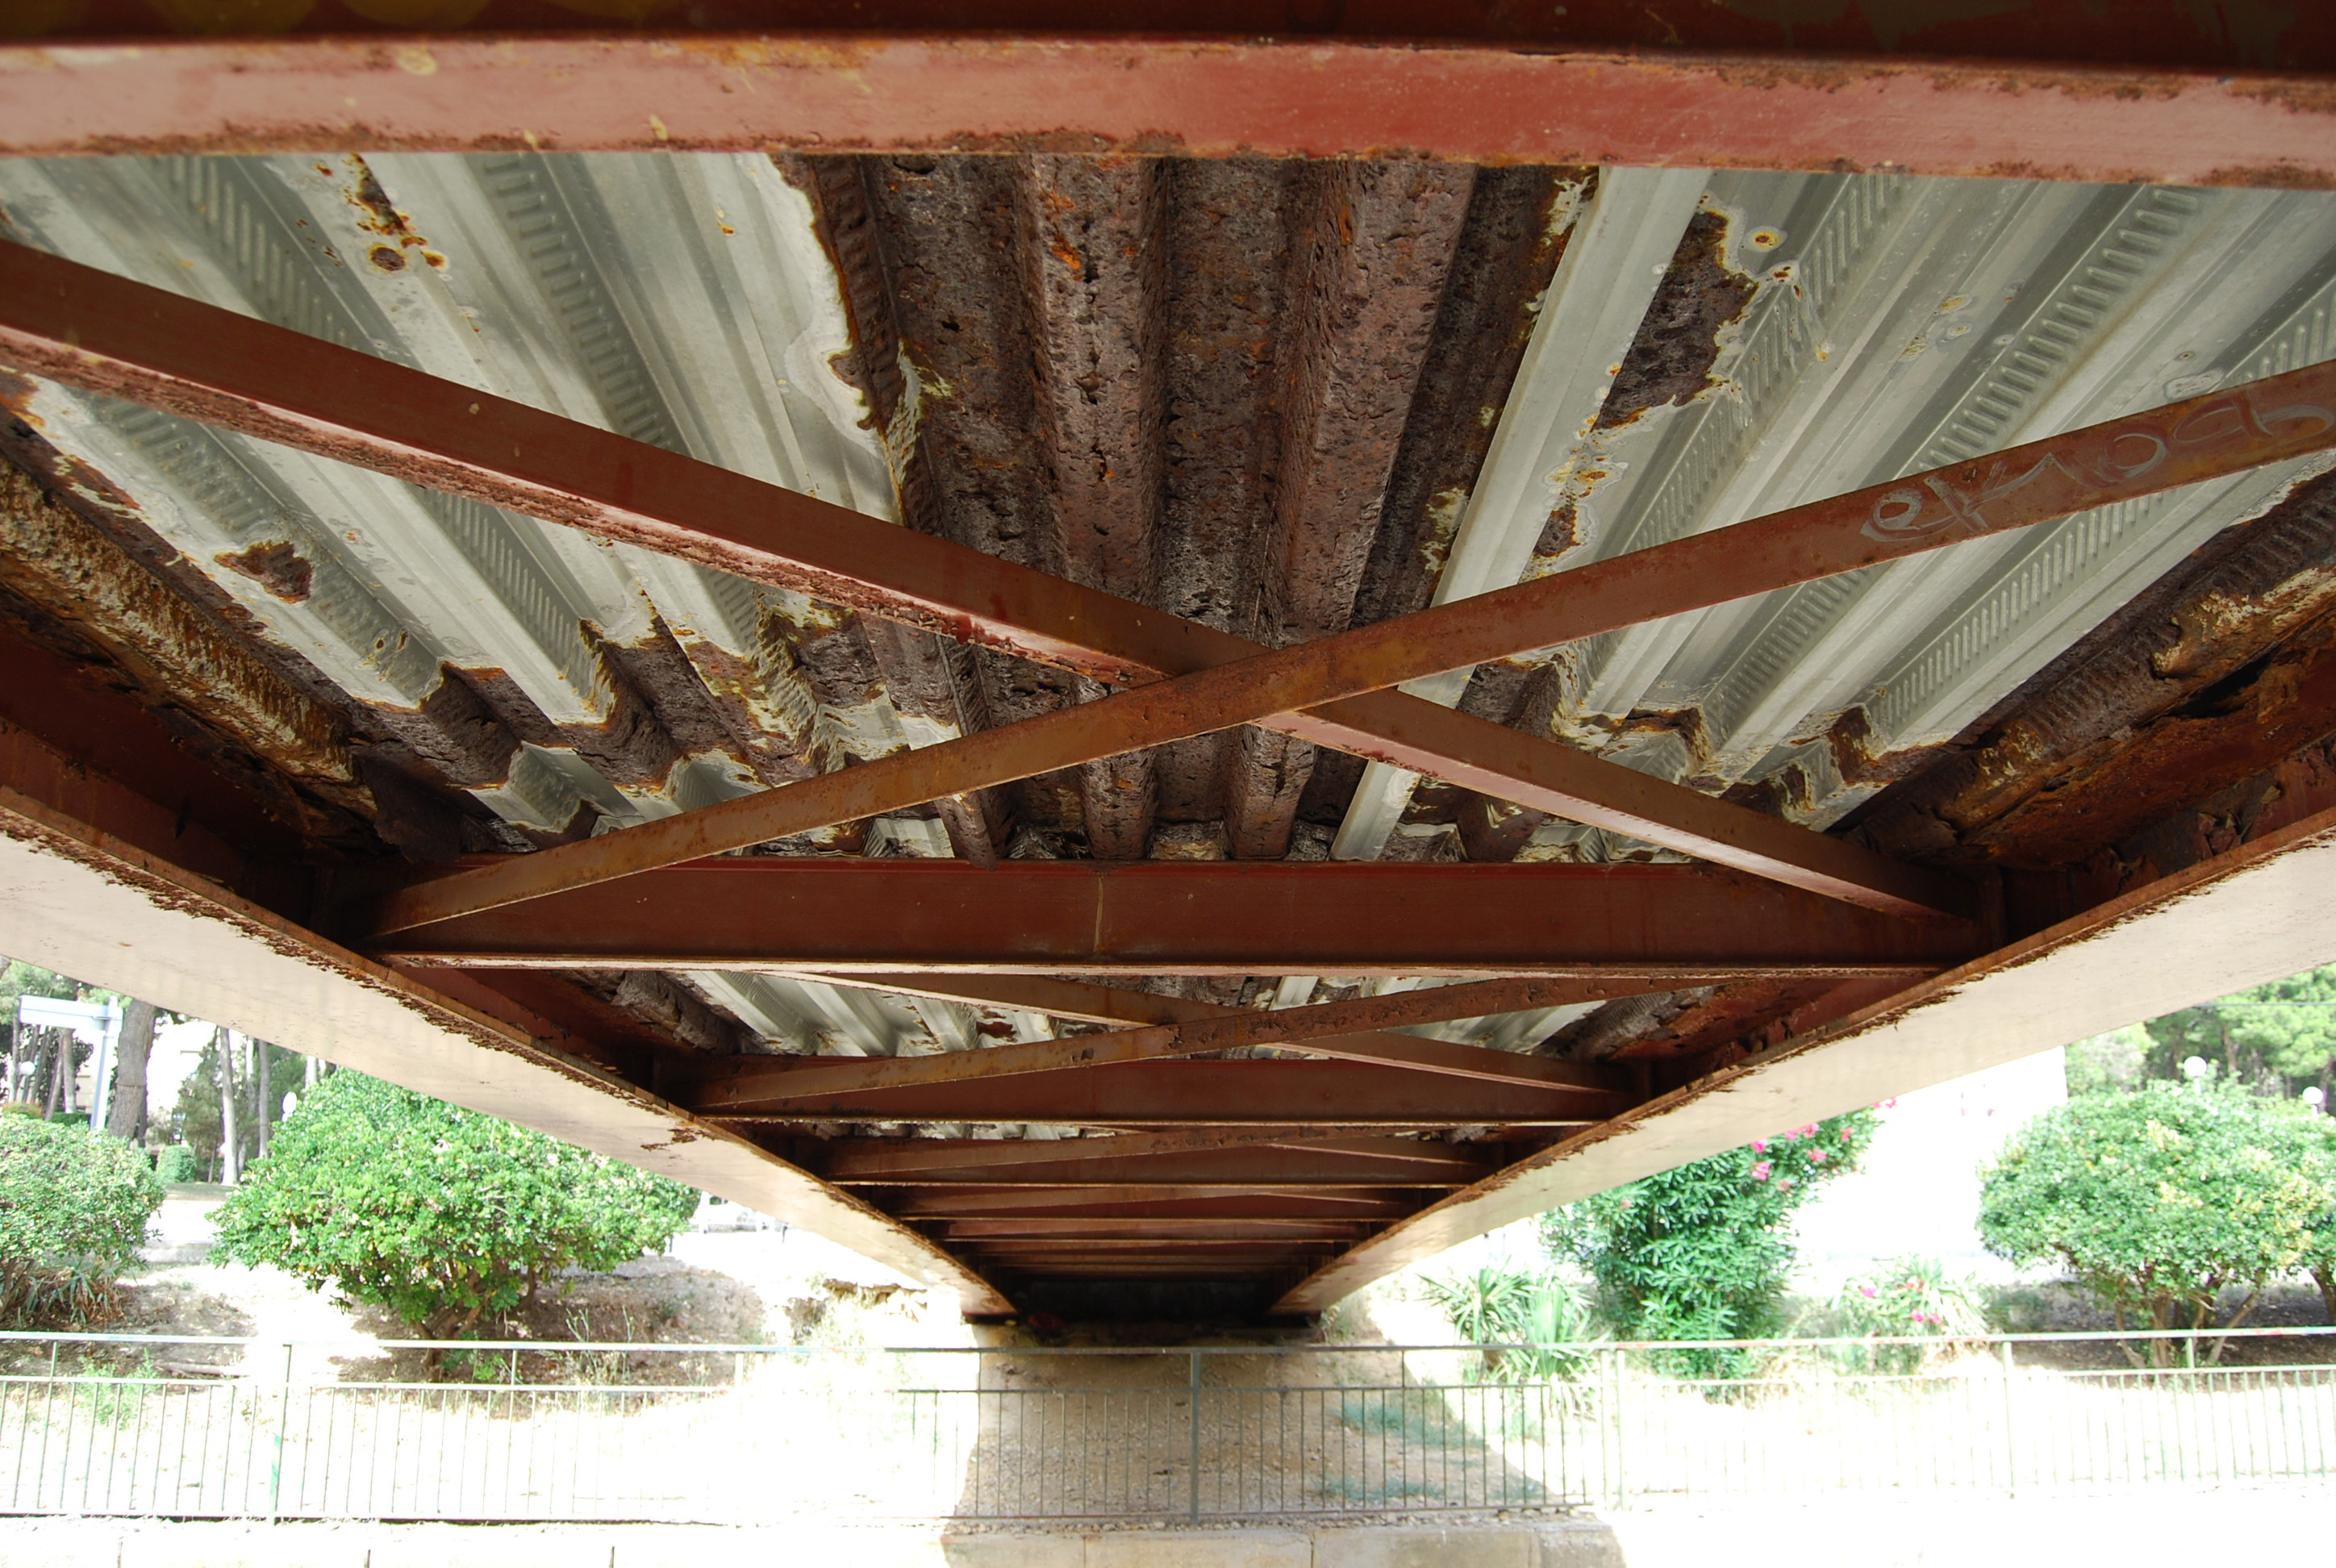
\includegraphics[width=\textwidth]{figures/corrosion_fisura_transversal_zona_estribo_derecho}
  \caption{Corrosión en chapa colaborante de forjado.}
  \end{subfigure}
\hfill
  \begin{subfigure}[r]{\widhtRightCol}
  \centering
  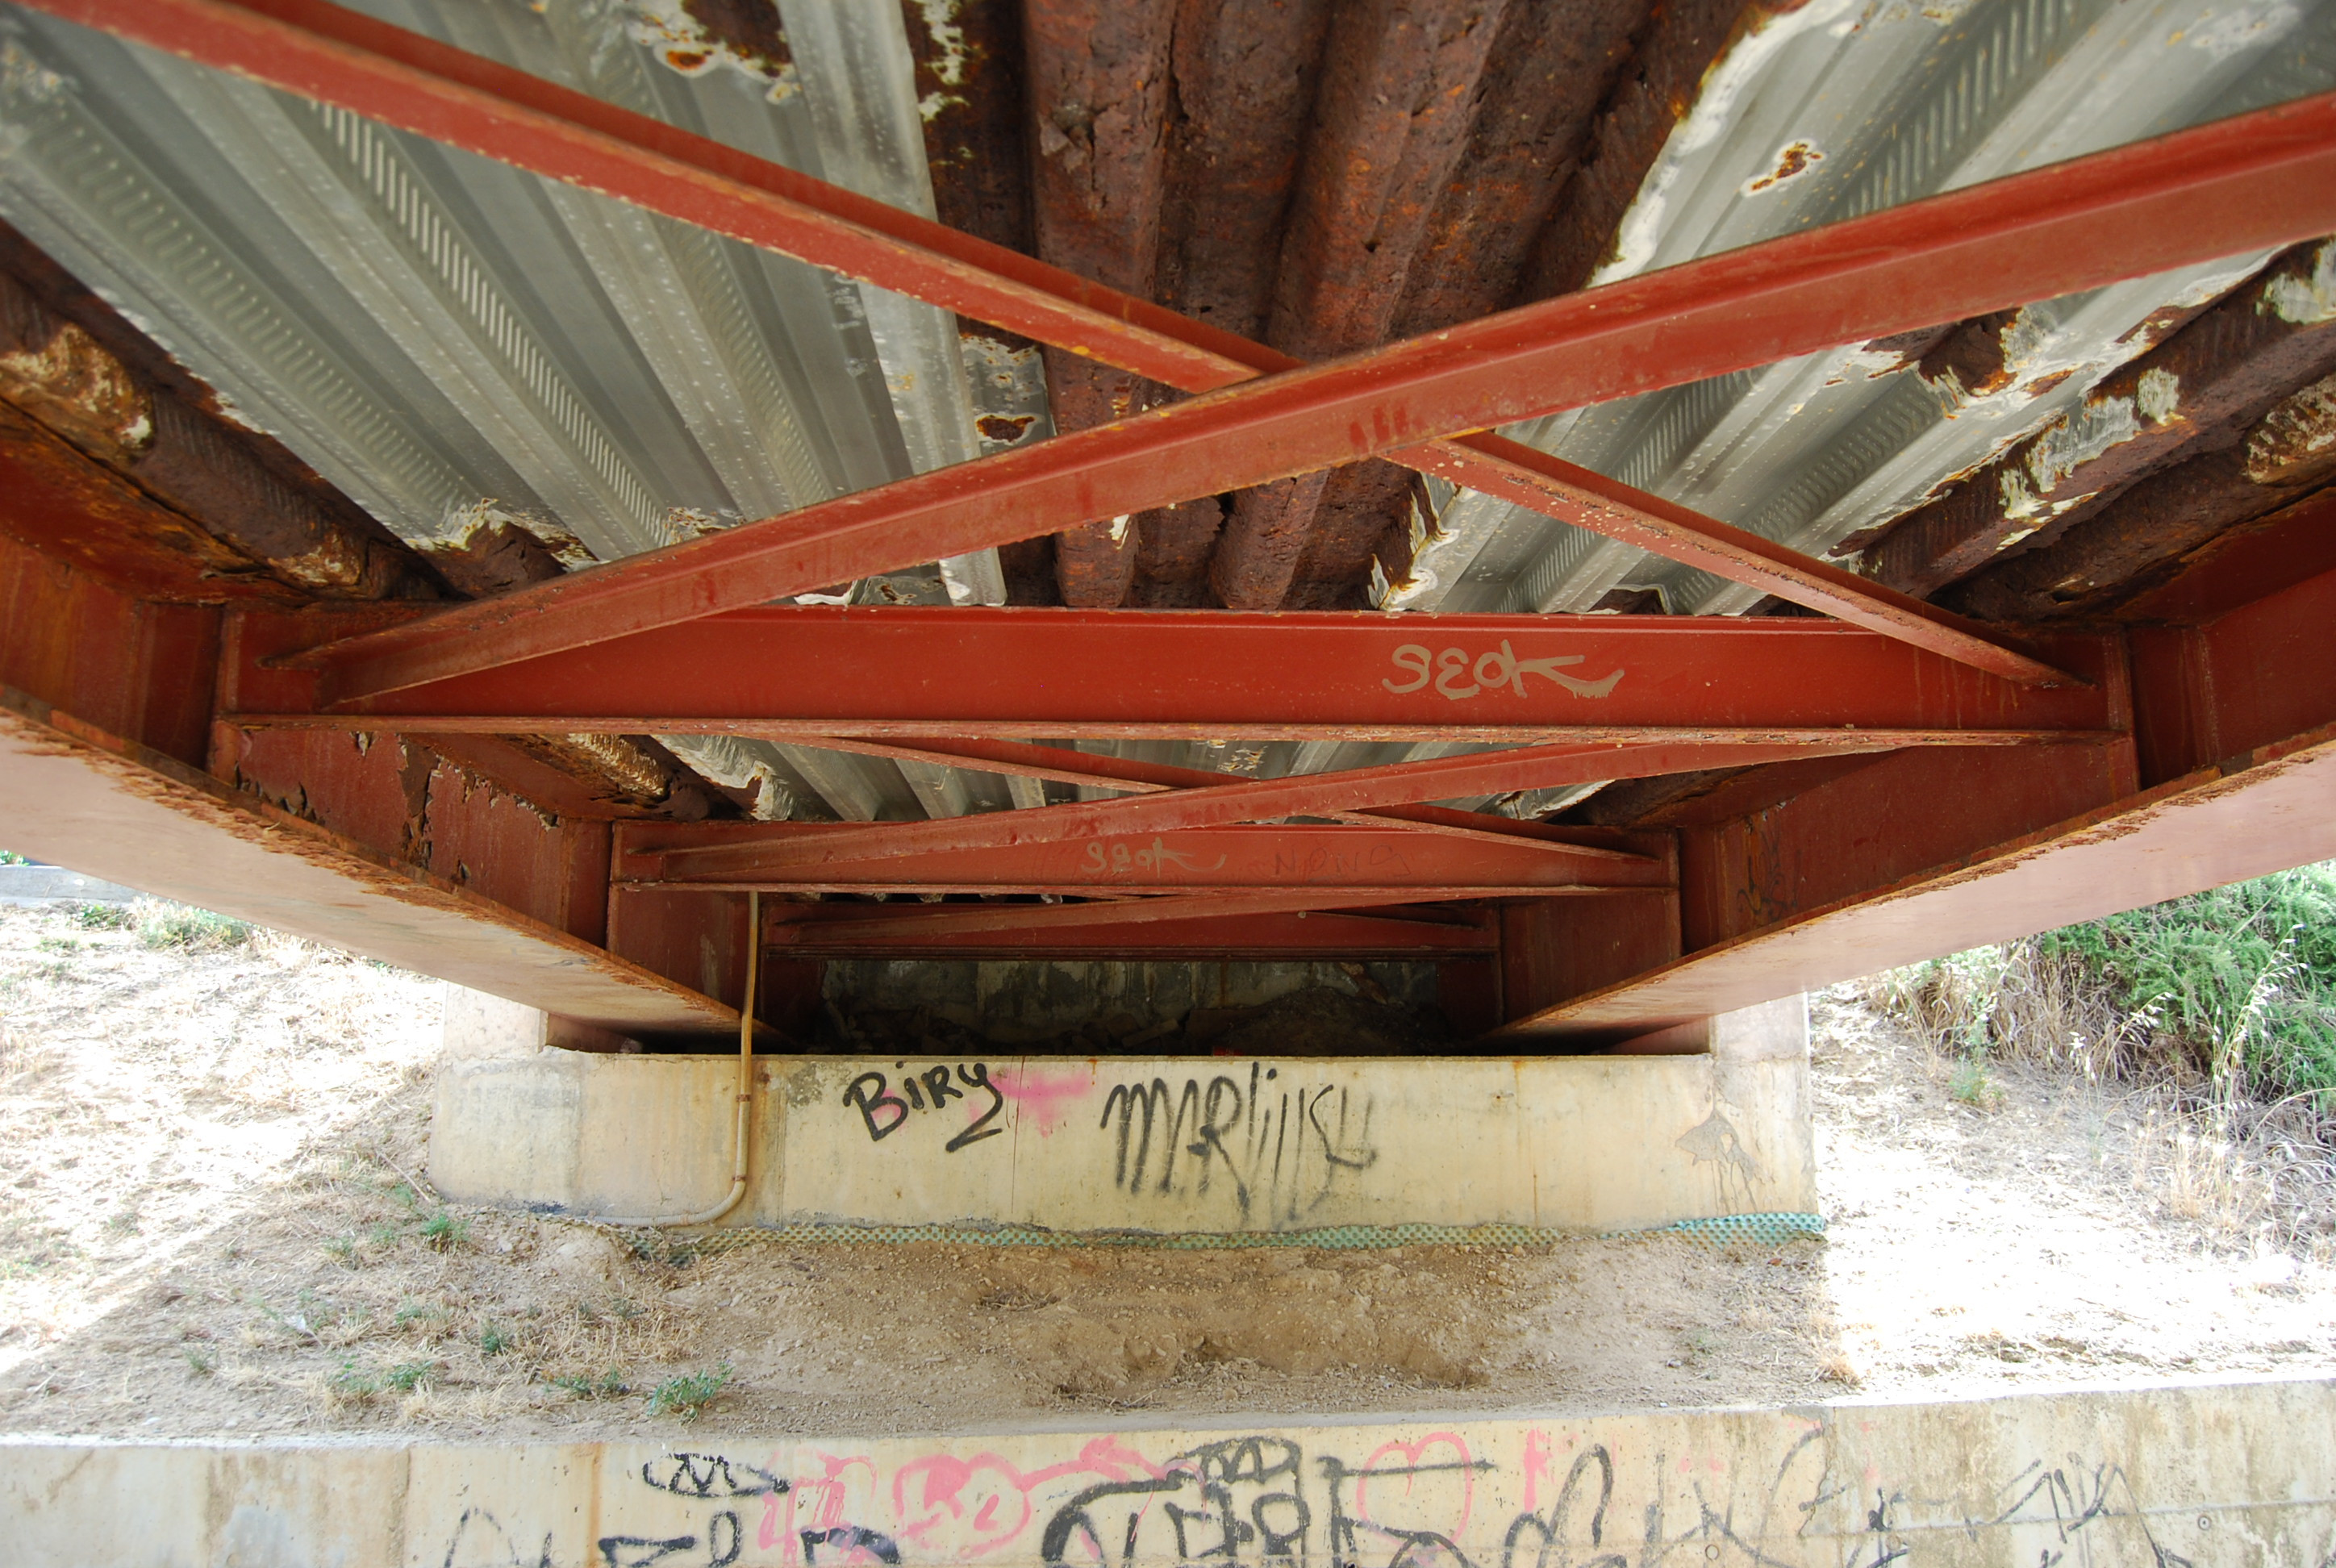
\includegraphics[width=\textwidth]{figures/corrosion_forjado_zona_central_y_laterales}
  \caption{Vista del estribo derecho y corrosión en forjado}
  \end{subfigure}
  \end{figure}


  %%  \begin{wrapfigure}{l}{\widhtLeftCol}
  %% \includegraphics[width=\widhtLeftCol]{figures/viaducto_segovia}
  %%  \caption{Viaducto de Segovia (Madrid)}\label{fg_viaducto_segovia}
  %%  \end{wrapfigure}
  %%  \emph{The New Amsterdam Theatre is a Broadway theater on 214 West 42nd Street, in the Theater District of Manhattan in New York City. It was one of the first Broadway venues to open in the Times Square neighborhood, on October 26, 1903. The theater has 1,702 seats across three levels. Both the Beaux-Arts exterior and the Art Nouveau interior of the building are New York City}



   
   \begin{Parallel}{\widhtLeftCol}{\widhtRightCol}
     \ParallelLText{
       En el estudio de soluciones se  valoraron y compararon tres soluciones de reparación de la estructura y tres de sustitución del tablero. Las primeras consistenten en la demolición del forjado de chapa colaborante, protección de la estructura metálica con sistema de pintura adecuado, y ejecución de nuevo forjado en madera, trámex o forjado mixto, resepectivamente. Se planteó la sustitución del tablero por celosía metálica,en acero al carbono y acero inoxidable. Finalmente, se estudió la solución de sustituir el tablero con estructura de madera y diafragmas de acero inoxidable, resultado ser ésta la alternativa seleccionada por la Propiedad.
  }
 
  \ParallelRText{

   \emph{ In the preliminary project  study, three solutions to repair the structure and three to replace the deck were evaluated and compared. The first ones consist of the demolition of the collaborating sheet metal floor, protection of the metallic structure with an adequate painting system, and execution of a new wooden floor, tramex or mixed floor, respectively. Regarding the replacement solutions, the substitution by a metal lattice deck, in carbon steel or stainless steel, was proposed. Finally, the solution of replacing the deck by a wooden structure with stainless steel diaphragms was studied, which turned out to be the alternative selected by the client.}


  }

  \begin{figure}[b]
  \begin{subfigure}[l]{\widhtLeftCol}
  \centering
  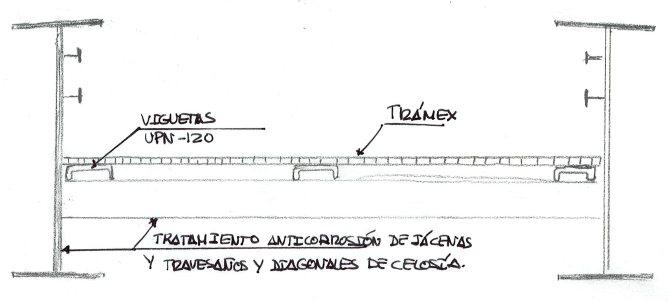
\includegraphics[width=\textwidth]{figures/forjado_tramex}
  \caption{Solución de reparación de la estructura principal del tablero y nuevo forjado de trámex}
  \end{subfigure}
\hfill
  \begin{subfigure}[r]{\widhtRightCol}
  \centering
  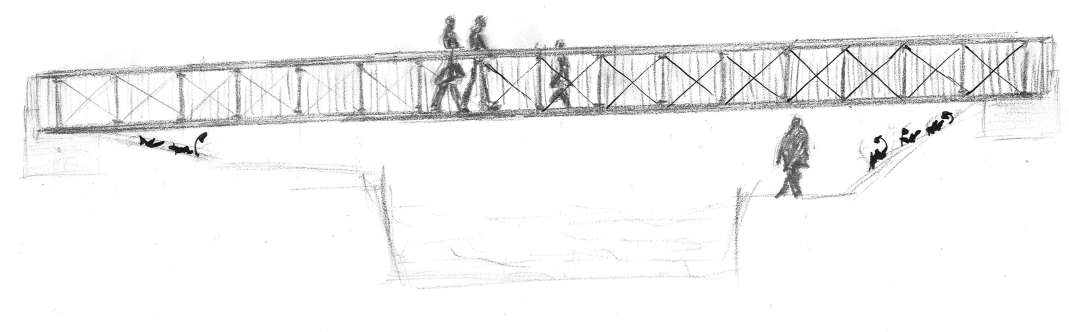
\includegraphics[width=\textwidth]{figures/sol_metalica_alzado}
  \caption{Solución de sustitución de tablero con celosía metálica.}
  \end{subfigure}
  \end{figure}

  \ParallelPar
  \ParallelLText{
    La pasarela proyectada está formada por un puente de vigas de tablero inferior. Las dos vigas de madera que forman los parapetos están unidas por diafragmas metálicos con forma de «U», que sirven de soporte al tablero y coartan el desplazamiento lateral de las vigas.
    
    Uno de los principales objetivos del diseño adoptado es aprovechar en lo posible lo ya construido, reduciendo, por tanto, los recursos empleados en la construcción y las molestias a los ciudadanos durante el desarrollo de las obras. En ese sentido, se ha procurado que la nueva estructura sea compatible con la disposición de los apoyos de la existente de modo que la operación de sustitución del tablero sea rápida y sencilla.
    
    También se procuró una buena integración de la estructura con el entorno. La afección al cauce del río Isuela es nula, puesto que se conserva el gálibo hidráulico. Otro tanto puede decirse respecto al tráfico peatonal bajo la misma. En cuanto a la integración estética, la pasarela se sitúa en un entorno con abundantes arbustos y árboles en las inmediaciones y amplias zonas verdes. Esto hace que el uso de la madera resulte natural en este contexto.
    
    
}
    \ParallelRText{

   \emph{The projected footbridge is formed by two wooden lower beams joined by "U"-shaped steel diaphragms, which serve as support for the deck and restrict the lateral movement of the beams.}
    
     \emph{One of the main objectives of the design is to make the most of what has already been built, thus reducing the resources used in the construction and the inconvenience to citizens during it. In this sense, particular care has been taken in ensuring that the new structure is compatible with the existing arrangement of  supports so that the operation of replacing the deck is quick and simple.}
    
     \emph{A good integration of the structure with the environment was also sought. The affectation to the course of the river Isuela is nil, since the hydraulic gauge is preserved. The same can be said regarding the pedestrian traffic under it. In terms of aesthetic integration, the footbridge is located in an environment with abundant bushes and trees in the immediate vicinity and extensive green areas. This makes the use of wood seem natural in this context.}
  }
   \end{Parallel}

\begin{figure}[h]
  \begin{subfigure}[l]{\widhtLeftCol}
  \centering
  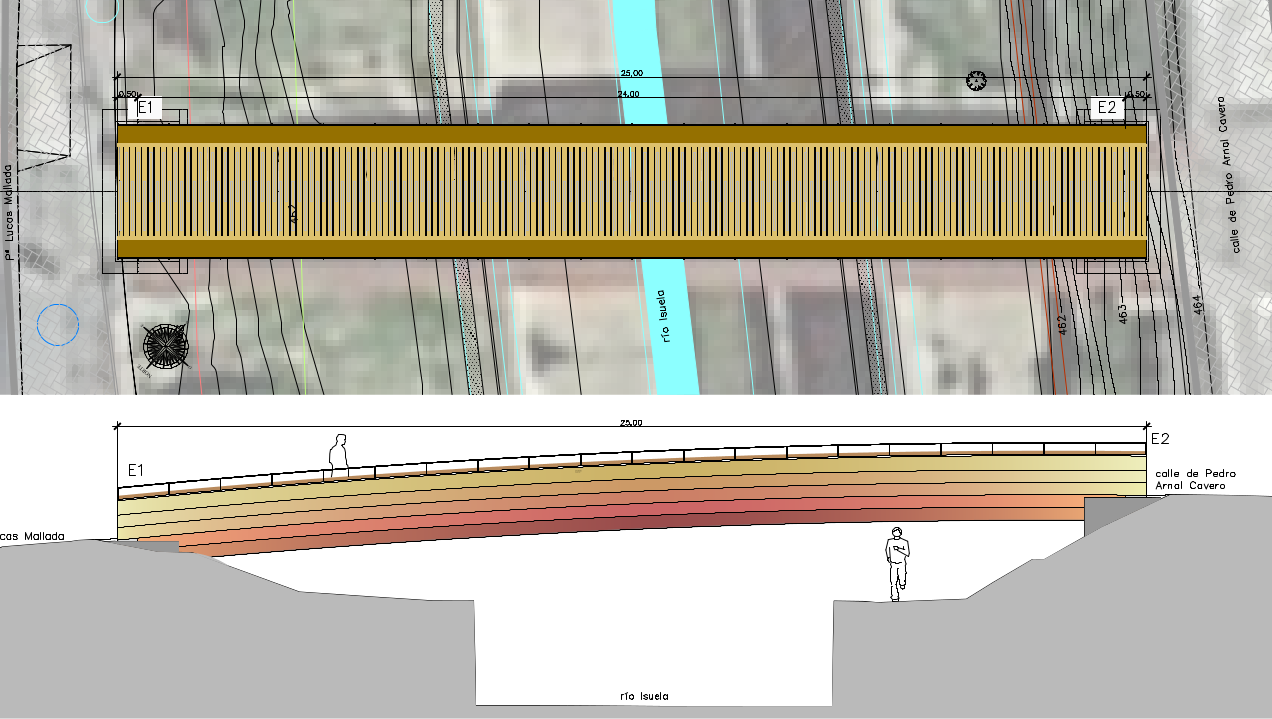
\includegraphics[width=\textwidth]{figures/planta_alzado}
  \caption{Planta y alzado desde aguas arriba de la pasarela}
  \end{subfigure}
\hfill
  \begin{subfigure}[r]{\widhtRightCol}
  \centering
  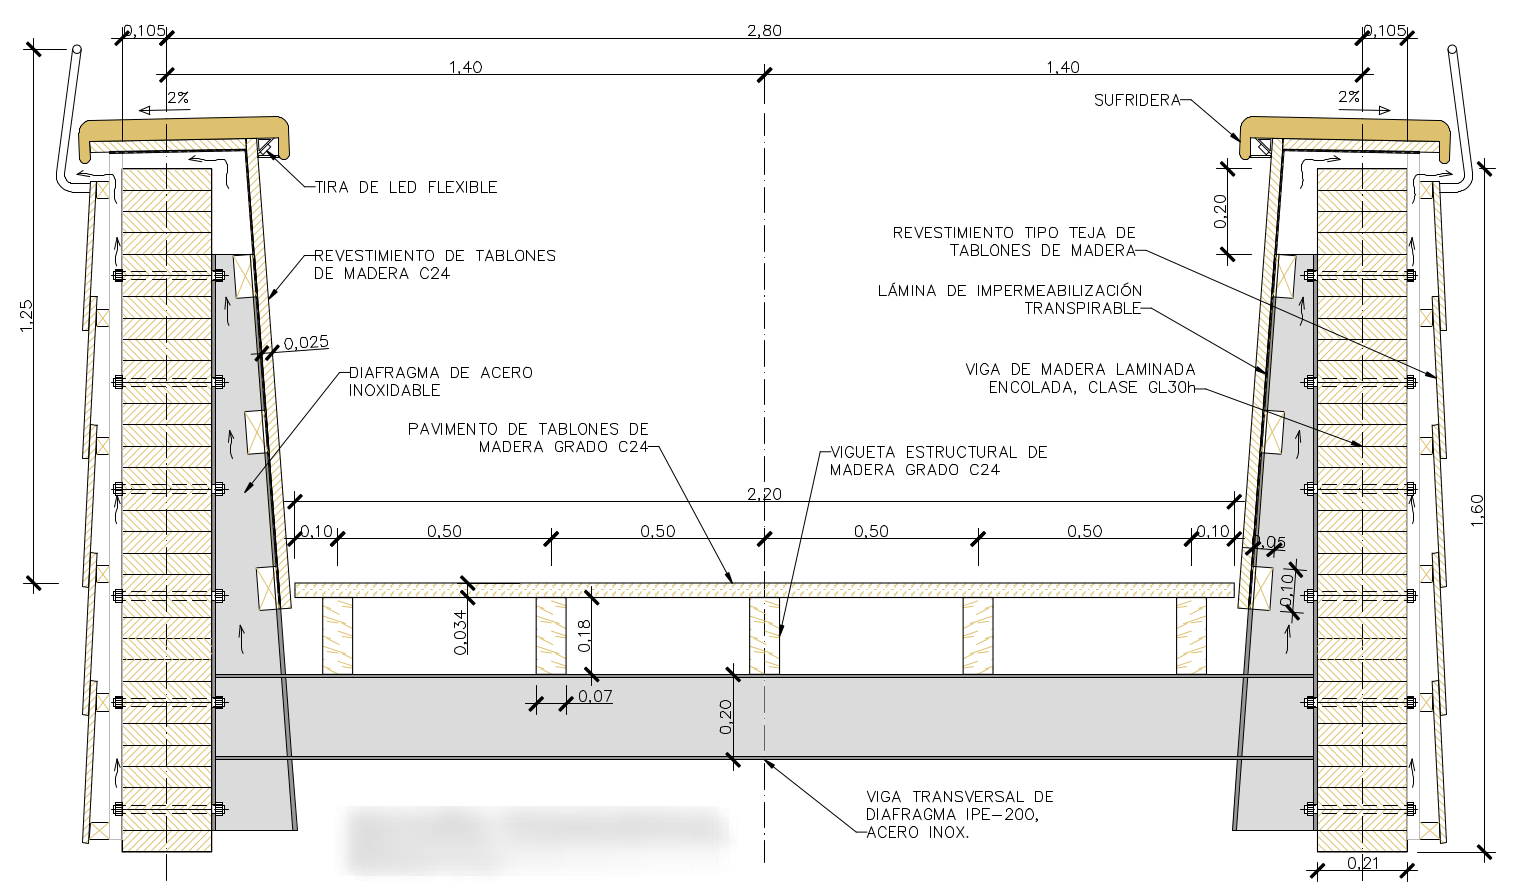
\includegraphics[width=\textwidth]{figures/sec_transv}
  \caption{Sección transversal del tablero}
  \end{subfigure}
  \end{figure}


   \begin{Parallel}{\widhtLeftCol}{\widhtRightCol}

  \ParallelLText{
    El tablero se compone de dos vigas de madera laminada encolada de 21 cm de ancho y 1,60 m de canto. Estas vigas están unidas por diafragmas transversales cada 2,4 m. El anclaje de los diafragmas a las vigas se hace mediante bulones de acero. El tablero propiamente dicho está formado por una serie de vigas rastrel longitudinales que apoyan en los diafragmas metálicos antes citados y que, a su vez, soportan la tablazón formada por piezas de 34 mm de espesor y 140 mm de ancho. Las viguetas tienen 70 mm de ancho y 180 mm de canto.
    
    La rigidez de la pasarela frente a cargas horizontales (viento) se consigue disponiendo un sistema de arriostramiento situado bajo el tablero y formado por cruces de San Andrés que unen las esquinas inferiores de los diafragmas en «U» consecutivos. Este arriostramiento está formado por redondos de acero inoxidable de 12 mm de diámetro. El cruce entre estos tirantes de acero inoxidable se resuelve mediante una pieza especial y la conexión con los perfiles metálicos mediante orejetas de acero inoxidable. Los tirantes dispondrán de un manguito tensor que permitirá ajustar el tesado del mismo.

    En general, se pretende evitar la aparición de zonas en las que puedan presentarse acumulaciones de agua y favorecer una adecuada ventilación de los elementos de madera, mediante, por ejemplo, la disposición de juntas entre las distintas piezas o el redondeo de los cantos de las mismas.

    Los elementos estructurales de madera se tratan en profundidad en autoclave para clase de uso 3.2, con el nivel de protección frente a agentes bióticos NP3. La elección del acero inoxidable como material para los diafragmas obedece igualmente a la necesidad de prolongar la vida útil todo lo posible. La viga principal de madera laminada se protege frente a la acción directa de los agentes meteorológicos mediante la instalación de dos tipos de revestimiento: para la superficie interior, se elige un revestimiento con tablones de orientación vertical siguiendo la superficie ligeramente inclinada marcada por los diafragmas de acero. En el exterior, el revestimiento se forma con tablones orientados horizontalmente e inclinados respecto al paramento vertical, de forma que se solapan siguiendo un patrón de tipo teja. El revestimiento exterior tipo teja funcionará de forma natural como una barrera frente a la lluvia; la impermeabilidad del revestimiento interior se asegura adosando al mismo por su cara interior una lámina de impermeabilización transpirable, que permite el paso del aire pero no de la humedad. Adicionalmente, la superficie de madera expuesta se trata con un acabado superficial mediante lasur. La ventilación del contacto viga-revestimiento es fundamental para la durabilidad de la viga, que soporta la función estructural principal, para evitar que se produzcan acumulaciones de humedad y ataque por agentes bióticos. Se provee por esta razón a la sección transversal en dicho contacto de una cámara de aire con aberturas en la parte inferior y superior.
}

  \ParallelRText{
     \emph{The deck is made up of two glued laminated wood beams 21 cm wide and 1.60 m deep. These beams are joined by transverse stainless steel diaphragms every 2.4 m. The anchoring of the diaphragms to the beams is done by means of steel bolts. The floor  is made up of wood joists, 70 mm wide and 180 mm deep, that rest on the aforementioned steel diaphragms and which, in turn, support the decking floorboard pavement made up of pieces 34 mm thick and 140 mm wide}
    
     \emph{The footbridge's stiffness against horizontal loads (wind) is achieved by arranging a bracing system located under the deck and made up of crosses that join the lower corners of the consecutive "U" diaphragms. This bracing is made up of 12 mm diameter stainless steel rods. The crossing between these stainless steel braces is resolved by means of a special piece and the connection with the metal profiles by means of stainless steel lugs. The braces will have a sleeve that will allow adjusting its tensioning.}

     \emph{In general, the aim is to avoid the appearance of areas where water accumulations may occur and to promote adequate ventilation of the wooden elements, through, for example, the arrangement of joints between the different pieces or the rounding of the edges of the same.}

     \emph{The wooden structural elements are thoroughly treated in an autoclave for use class 3.2, with the level of protection against biotic agents NP3. The choice of stainless steel as a material for the diaphragms is also due to the need to prolong the useful life as much as possible.The main beam of laminated wood is protected against the direct action of weather agents by installing two types of cladding: for the interior surface, a cladding with vertically oriented planks is chosen, following the slightly inclined surface marked by the diaphragms of steel. On the outside, the cladding is formed with planks oriented horizontally and inclined with respect to the vertical face, so that they overlap following a tile-like pattern. The tile-like exterior cladding will naturally function as a barrier against rain; the waterproofing of the inner lining is ensured by attaching a breathable waterproofing sheet to it on its inner face, which allows the passage of air but not humidity. Additionally, the exposed wooden surface is treated with a surface finish using lasur. The ventilation of the beam-cladding contact is essential for the durability of the beam, which supports the main structural function, to prevent moisture accumulation and attack by biotic agents. For this reason, the cross-section at said contact is provided with an air chamber with openings at the bottom and at the top.}
  }
  
\end{Parallel}


    \end{document} 

